\documentclass[12pt]{article}
\usepackage{amsmath}
\usepackage{graphicx}
\usepackage[export]{adjustbox}
\usepackage[left=2cm, right=2cm, top=2.5cm, bottom=2.5cm]{geometry}

\title{IoT - Challenge 1}
\author{Raul Agolli}
\date{March 2026}

\begin{document}

\maketitle
\newpage

\section{Topic}
This project focuses on the design, implementation, and energy optimization of a wireless IoT sensor node. Built using an ESP32 microcontroller, a PIR motion sensor, and an analog photoresistor, the device monitors room occupancy and ambient luminosity to support automated smart home lighting decisions.

\section{Hardware Architecture and Pin Configuration}

\noindent
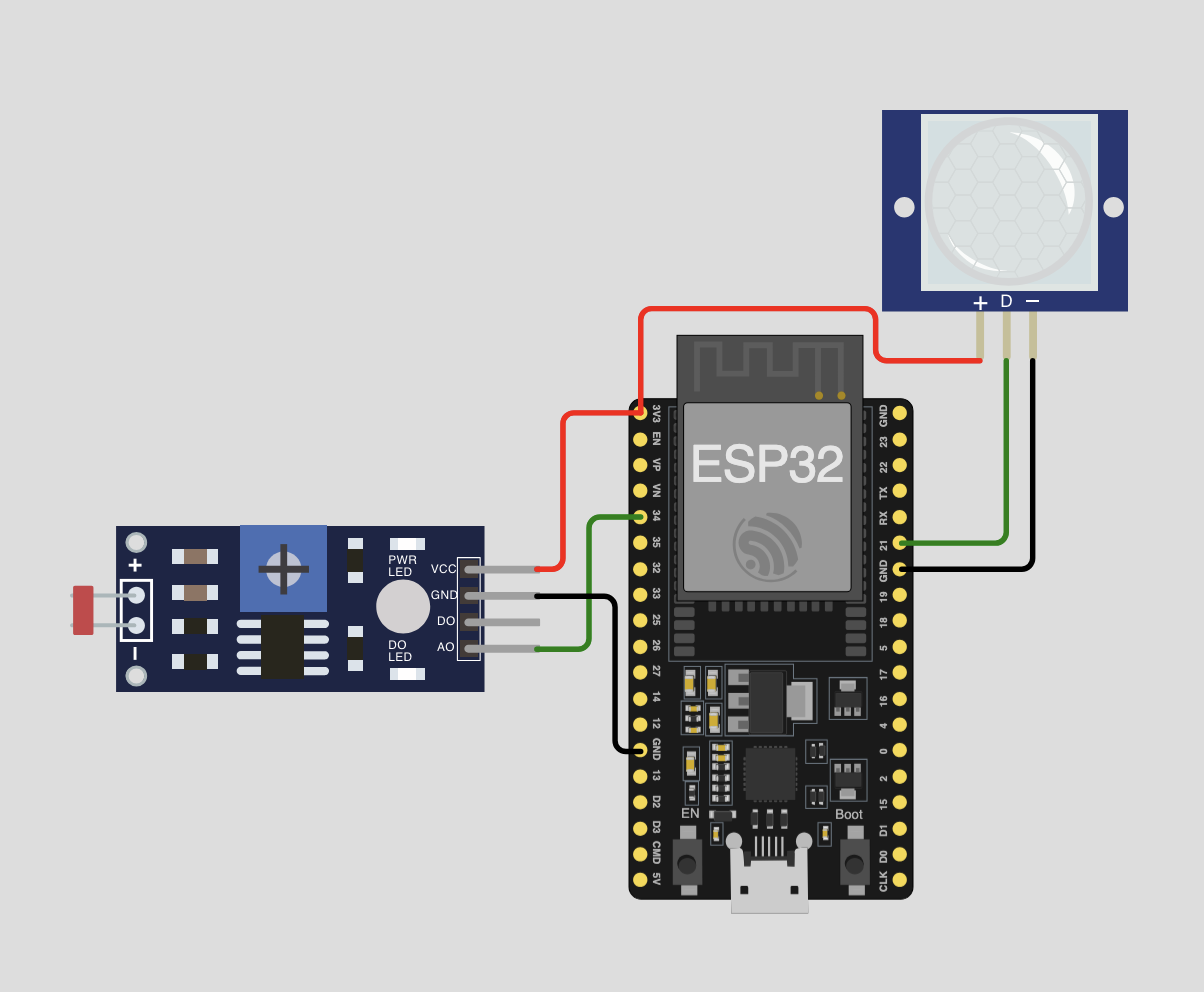
\includegraphics[width=0.48\linewidth, valign=t]{schematics.png}
\begin{minipage}[t]{0.48\linewidth}
The sensor node is built around an ESP32 microcontroller. 
Environmental monitoring is achieved using a standard PIR motion sensor to detect occupancy and an analog photoresistor (LDR) to measure ambient luminosity. Both components are powered exclusively from the ESP32’s 3.3V (3V3) pin.
\end{minipage}
\\

\textbf{Pin 34 (Photoresistor):} The LDR requires an Analog-to-Digital Converter (ADC) to translate varying light levels into readable data. Pin 34 is a dedicated ADC1, input-only pin.

\textbf{Pin 21 (PIR Sensor): }The motion sensor outputs a simple digital binary state (HIGH for motion, LOW for empty). Pin 21 is utilized as a standard general-purpose input/output (GPIO) pin.

\section{Code Review}

\noindent
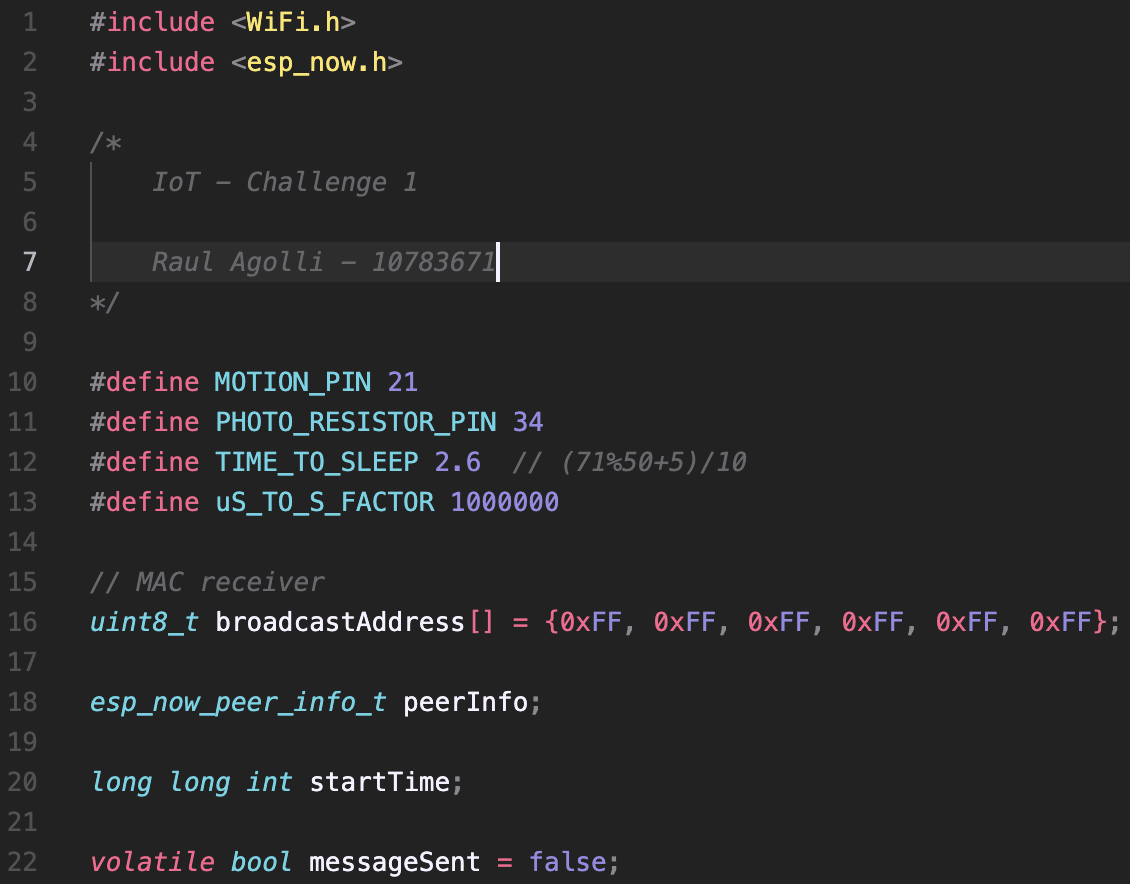
\includegraphics[width=0.48\linewidth, valign=t]{code1.png}
\begin{minipage}[t]{0.48\linewidth}
\textbf{Initial Configuration Block}\\
Imports the necessary Wi-Fi and ESP-NOW libraries, and maps the physical pins for the motion sensor (21) and photoresistor (34).\\
Defines the target destination as a broadcast MAC address (FF:FF:FF:FF:FF:FF) so the sink node can receive the data, and prepares the ESP-NOW peer structure.\\
Calculates the specific Deep Sleep duration (2.6 seconds) and initializes the messageSent flag.
\end{minipage}
\\

\noindent
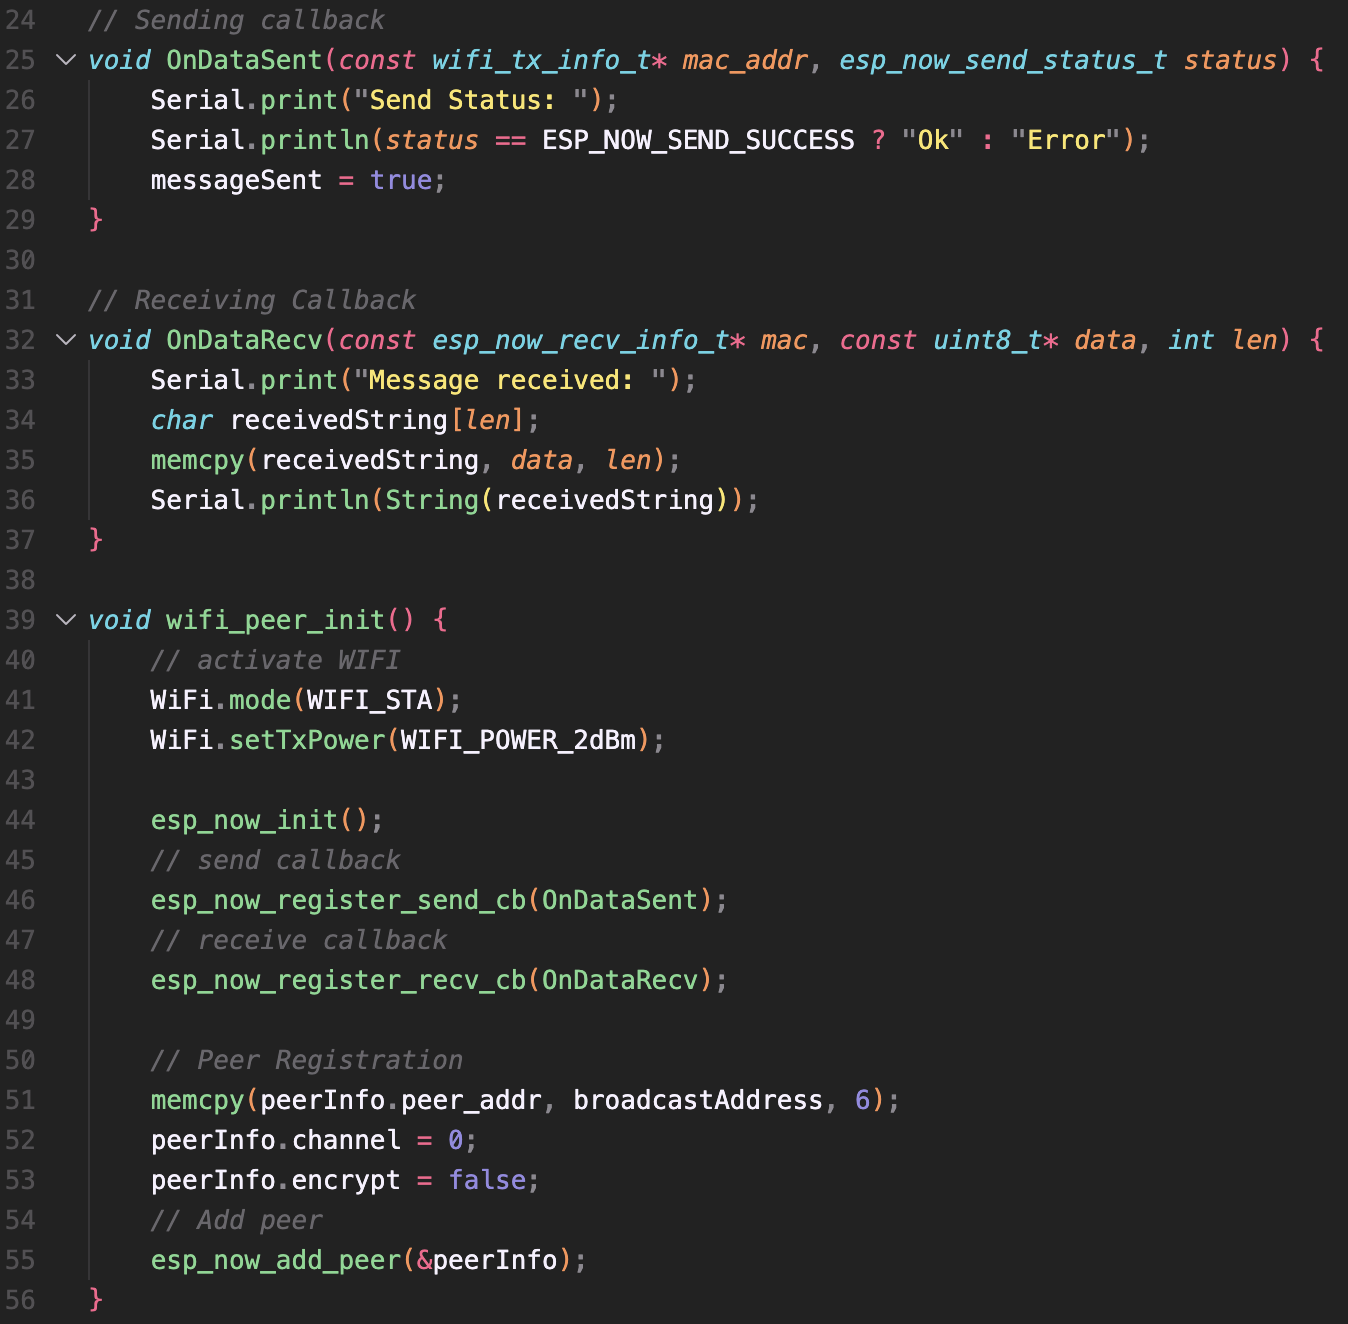
\includegraphics[width=0.48\linewidth, valign=t]{code2.png}
\begin{minipage}[t]{0.48\linewidth}
This section configures the ESP-NOW communication protocol. The \textbf{wifi\_peer\_init()} function initializes the Wi-Fi radio in Station mode, explicitly restricting the transmission power to 2dBm to minimize energy consumption, and registers the sink node's broadcast address as a peer. It also binds two asynchronous callback functions: \textbf{OnDataRecv} for handling incoming data, and \textbf{OnDataSent}, which is critically important because it updates the messageSent flag to confirm the payload has successfully left the antenna before the microcontroller is allowed to enter Deep Sleep.
\end{minipage}

\noindent
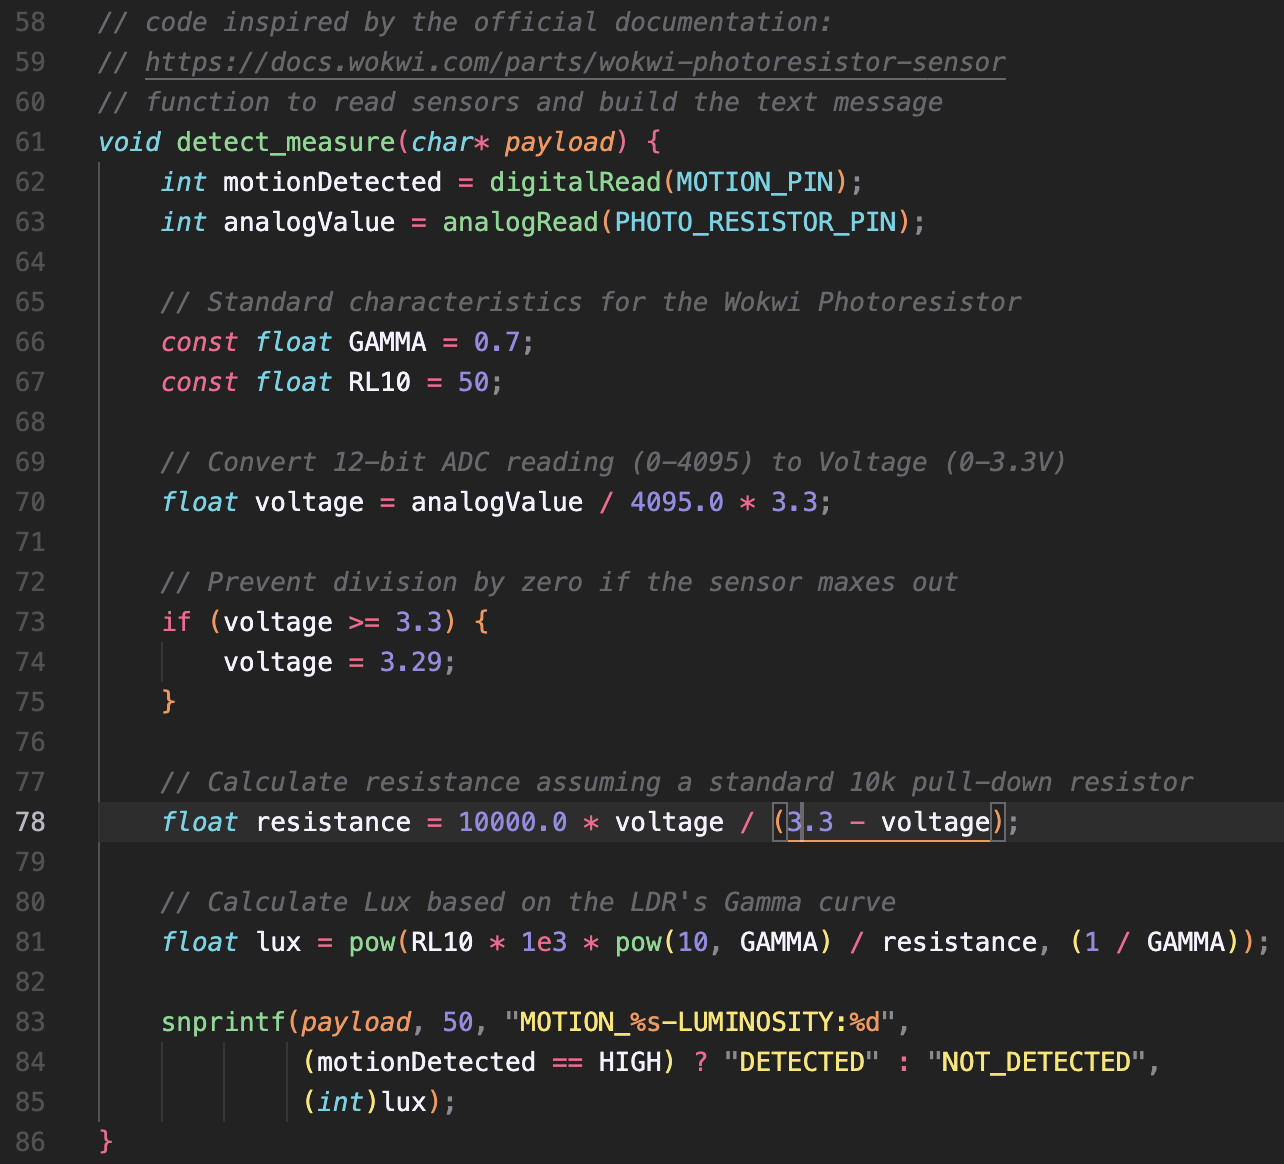
\includegraphics[width=0.48\linewidth, valign=t]{code3.png}
\begin{minipage}[t]{0.48\linewidth}
The \textbf{detect\_measure} function is responsible for sampling the environmental sensors and formatting the data payload. It reads the digital binary state of the PIR sensor and converts the raw analog voltage of the photoresistor into a standardized Lux value using the component's Gamma curve and resistance profile. To meet the strict assignment formatting requirements, it concatenates these readings into a single structured message (e.g., MOTION\_DETECTED-LUMINOSITY:450).\\
This function constructs the payload using a single \textbf{snprintf}. This avoids heap memory fragmentation.
\end{minipage}

\noindent
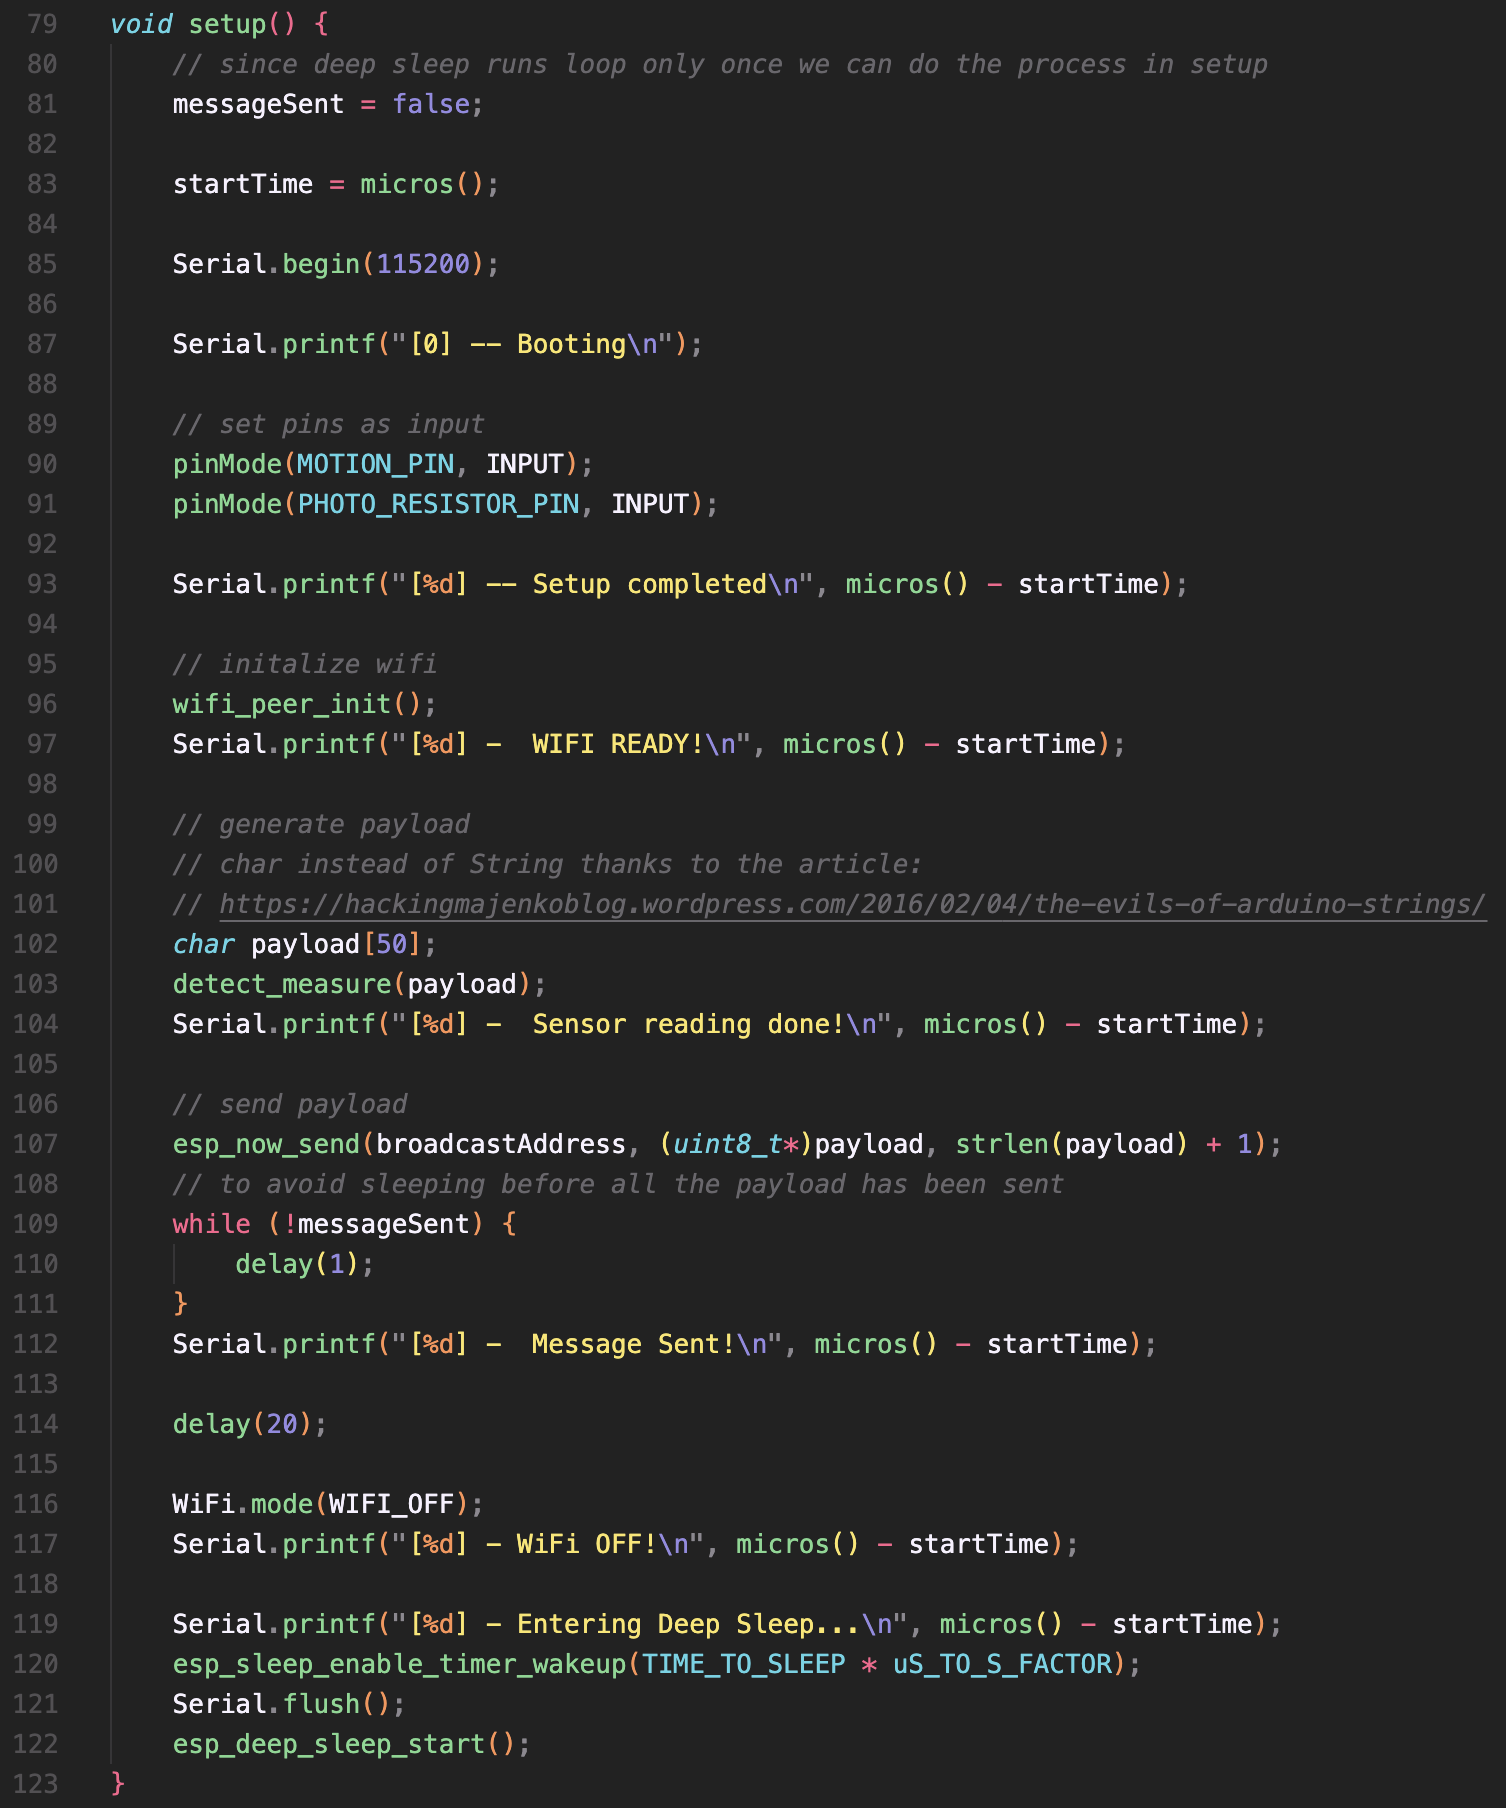
\includegraphics[width=0.48\linewidth, valign=t]{code4.png}
\begin{minipage}[t]{0.48\linewidth}
The \textbf{setup()} function orchestrates the complete lifecycle of the sensor node during its brief active window. Because Deep Sleep resets the microcontroller upon waking, the entire operational sequence is executed here rather than in the standard loop(). The function utilizes micros() to accurately log the duration of each operational phase, which provides the timing data needed for the system's energy profiling. It sequentially initializes the hardware and Wi-Fi, calls the sensor-reading function to build the memory-efficient payload, and transmits the data. Crucially, it employs a blocking while (!messageSent) loop to prevent a race condition, ensuring the Wi-Fi radio fully completes the ESP-NOW transmission before the system powers down the radio and transitions back into its calculated Deep Sleep state.
\end{minipage}

\newpage
\section{Sensor Calibration and ADC Quantization Error}
During testing, a minor deviation of roughly 5 to 10 Lux was observed between the environmental parameters set in the simulation and the microcontroller's final computed output. This discrepancy is a standard, expected artifact of Analog-to-Digital Conversion (ADC) quantization. The ESP32 utilizes a 12-bit ADC (yielding discrete integer values from 0 to 4095) to measure the analog voltage drop across the photoresistor's voltage divider circuit. Because the mathematical relationship between the LDR's electrical resistance and ambient illuminance follows an exponential power curve, a minimal change of just one or two discrete ADC steps translates into a disproportionately larger jump in the final Lux calculation, particularly at higher light intensities. This hardware-level quantization, combined with the truncation of floating-point variables into integers for payload transmission, perfectly accounts for this highly acceptable margin of error.

\section{Energy Consumption and Average Power Estimation}
For this part a Jupyter Notebook has been used, which can be found in the challenge directory \textbf{energy\_estimation}.

\subsection{Average Power Consumption}
The analysis is based on the provided CSV files. Data was filtered using threshold values which were estimated by plotting the given datasets.\\
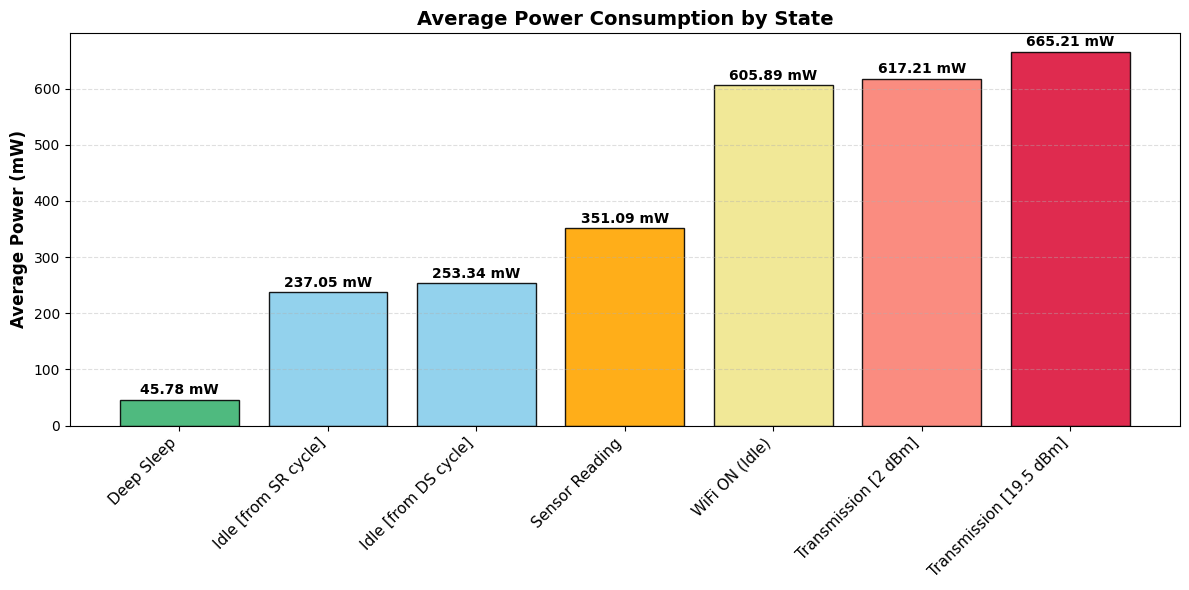
\includegraphics[width=1\linewidth, valign=t]{averagePowerByState.png}

\newpage
\subsection{Time Estimation}
To accurately estimate the duration of each operational phase, I utilized the ESP32’s micros() function. Because entering Deep Sleep causes the microcontroller to reset, a baseline startTime was recorded at the very beginning of the setup() function. This baseline was then subtracted at key execution milestones to print clean, relative timestamps.\\
Because software emulators like Wokwi can introduce slight timing variations depending on host CPU performance, relying on a single cycle is inaccurate. To mitigate this variance, I captured the serial output of 15 consecutive operating cycles into a structured dataset (timing.csv).\\
Using a Python script and the Pandas library, I calculated the exact time spent in each individual state by measuring the delta ($\Delta$t) between consecutive timestamps.\\
Finally, I averaged these durations across all recorded cycles to filter out emulator inconsistencies and establish a highly reliable time baseline for the final energy calculations.\\
The resulting average phase durations are reported below:\\\\
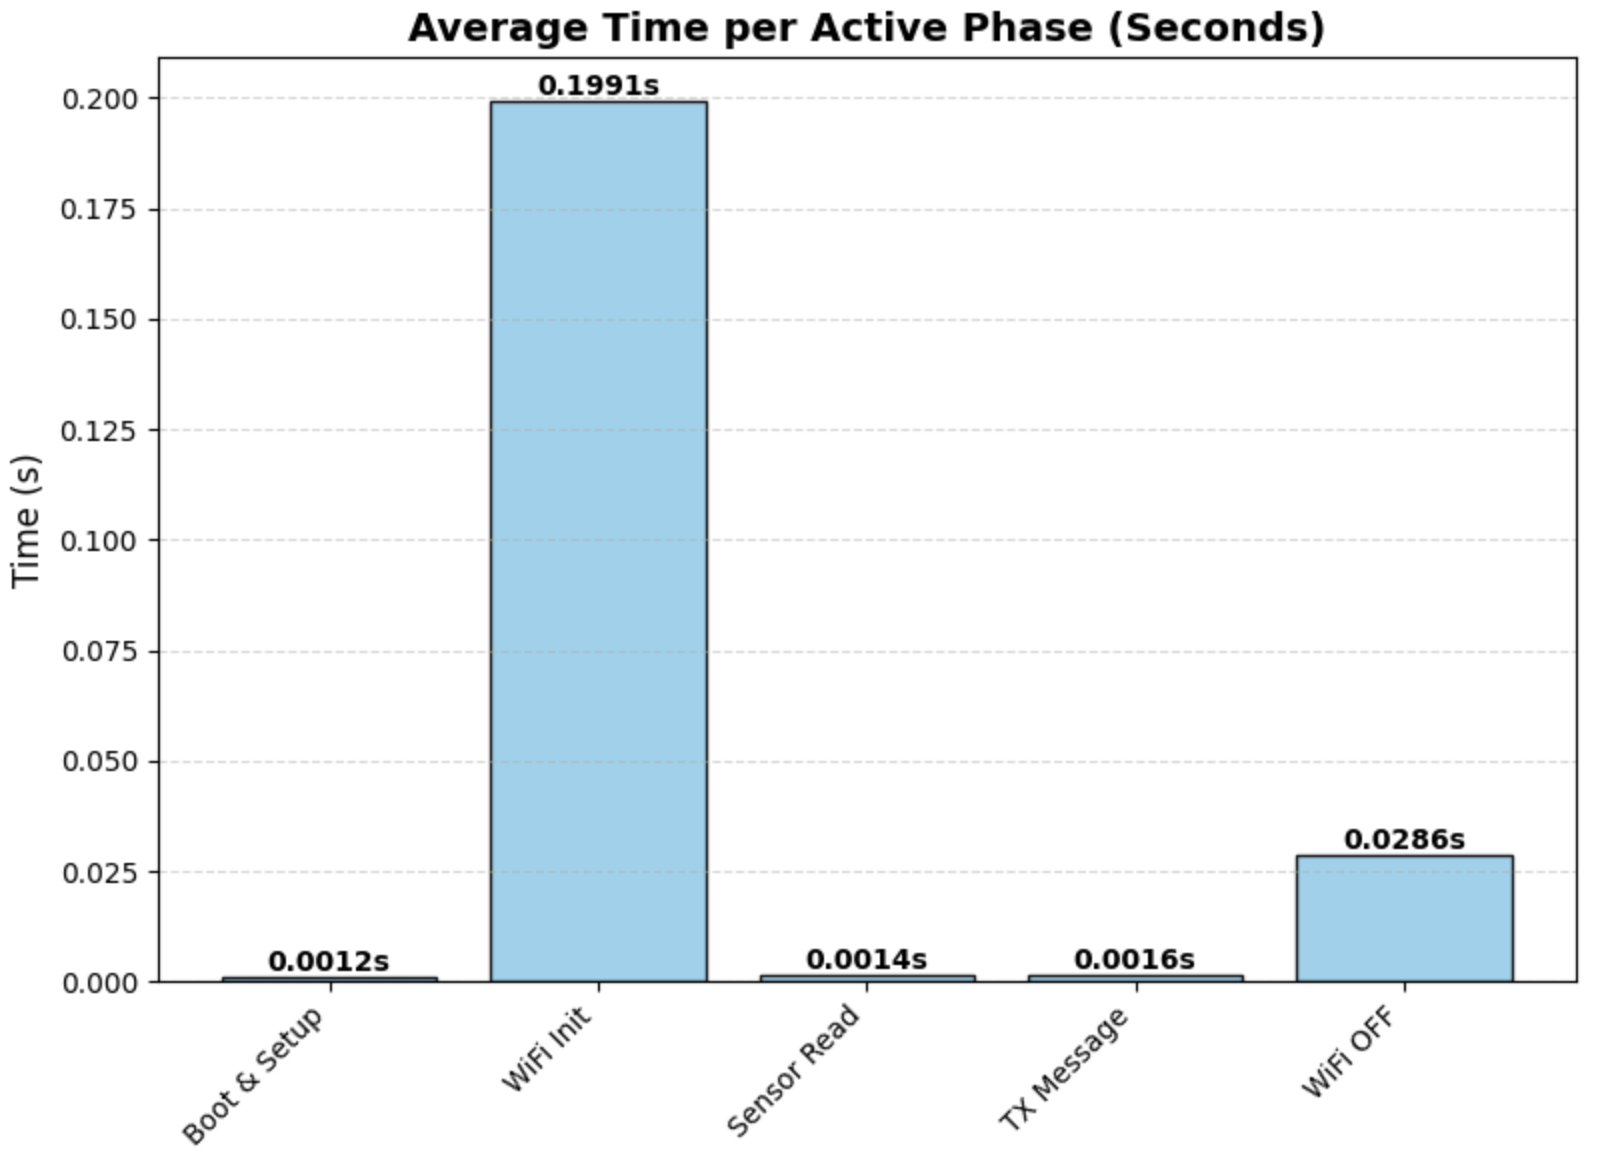
\includegraphics[width=1\linewidth, valign=t]{timePerPhase.png}
\\\\(Deep Sleep removed from the time chart so it doesn't ruin the scale for the tiny active phases.)\\

\subsection{Energy Estimation}
Given the time estimations and power consumptions obtained before, it’s possible to plot the average power per phase.\\
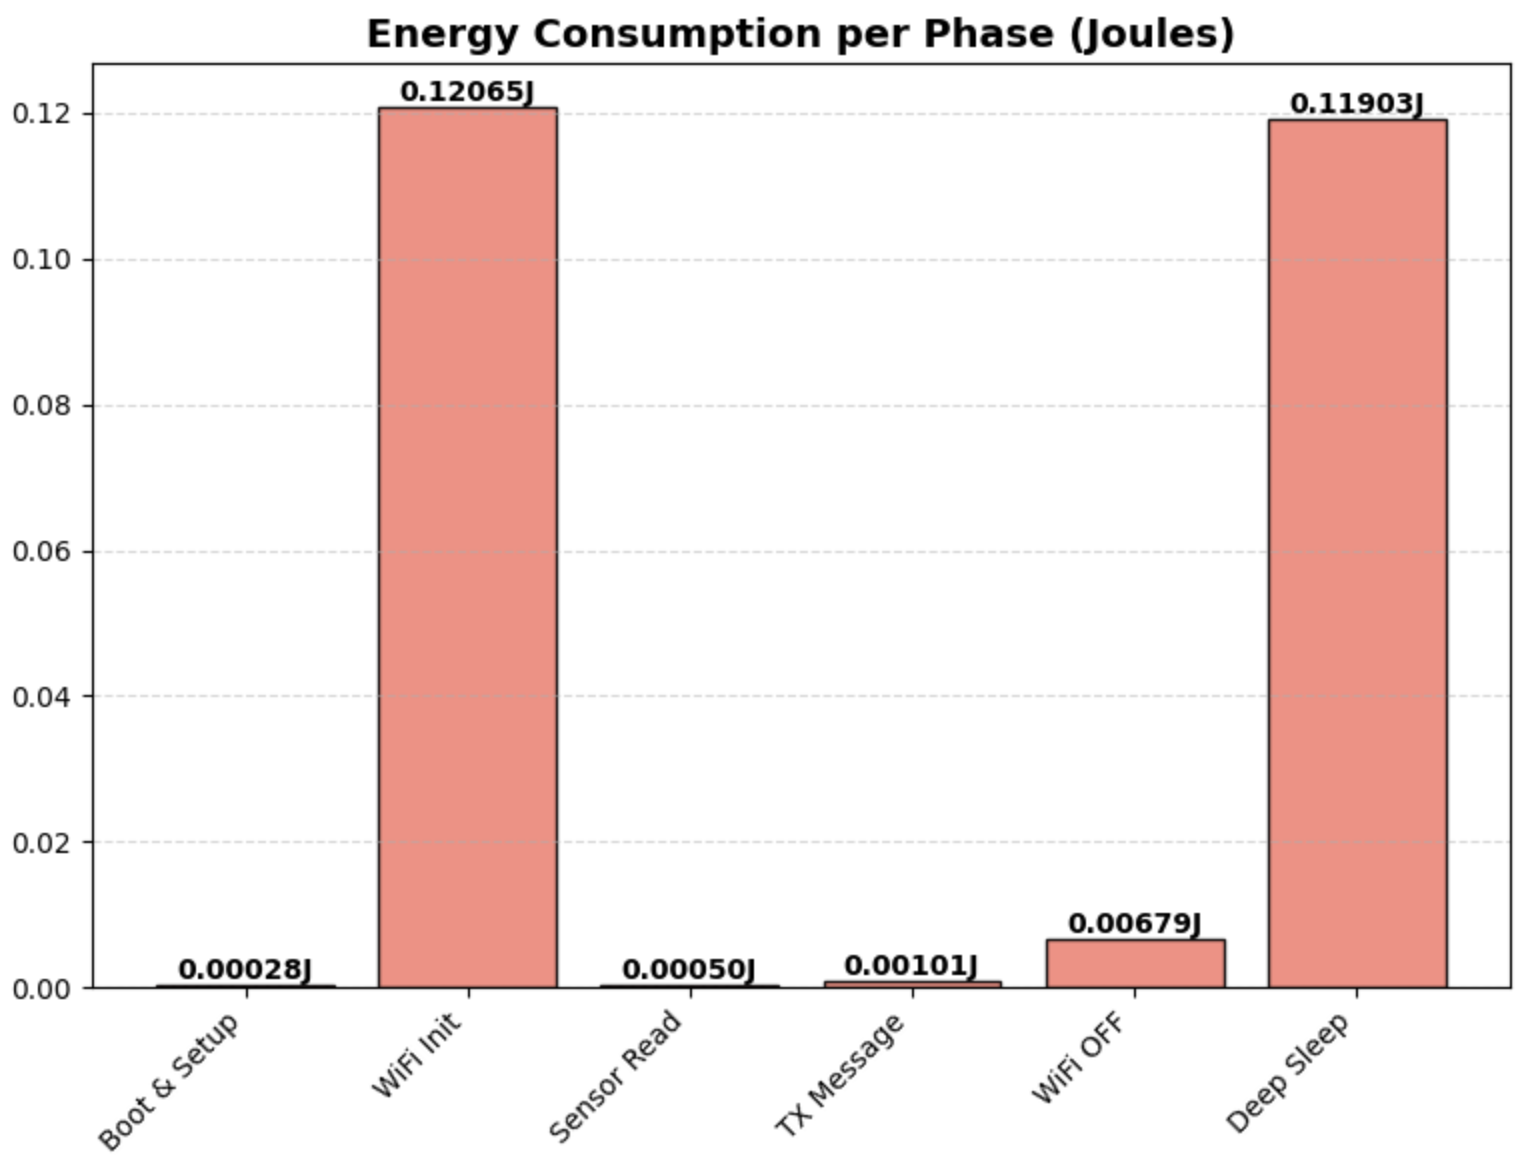
\includegraphics[width=1\linewidth, valign=t]{energyPerPhase.png}

\newpage
\subsection{Battery Life Estimation}
To evaluate the practical viability of the IoT sensor node, the total autonomous operating lifetime of the device was estimated. This estimation is based on the total available battery energy and the empirically calculated energy consumption of one complete operating cycle.

First, the total energy consumed per cycle ($E_{cycle}$) and the total duration of a single cycle ($T_{cycle}$) were computed by summing the respective values across all active and sleep phases (Booting, WiFi Initialization, Sensor Reading, Transmission, WiFi OFF, and Deep Sleep):

$$E_{cycle} = \sum_{i} E_{i}$$
$$T_{cycle} = \sum_{i} T_{i}$$

Next, the maximum number of complete operational cycles ($N_{cycles}$) the battery can sustain was determined by dividing the total available battery capacity ($E_{battery}$) by the energy consumed per cycle:

$$N_{cycles} = \frac{E_{battery}}{E_{cycle}}$$

Finally, the total estimated lifetime of the sensor node was calculated by multiplying the number of possible cycles by the duration of a single cycle. To provide a more intuitive and practical metric, this total lifetime in seconds ($L_{seconds}$) was subsequently converted into hours and days:

$$L_{seconds} = N_{cycles} \times T_{cycle}$$
$$L_{days} = \frac{L_{seconds}}{86400}$$

\subsubsection*{Empirical Results}
Applying the mathematical model to the simulated timing and power data yields the following baseline performance metrics for the sensor node:

\begin{itemize}
    \item \textbf{Total Battery Energy ($E_{battery}$):} 18671 Joules
    \item \textbf{Energy Consumed per Cycle ($E_{cycle}$):} 0.24825 Joules
    \item \textbf{Total Operational Cycles ($N_{cycles}$):} 75211 cycles
\end{itemize}

Based on these figures, the \textbf{Estimated Lifetime} of the sensor node is \textbf{59.17 hours}, or approximately \textbf{2.47 days}, before the battery is completely depleted.

\newpage
\section{Improvements}

\subsection{Delta reporting}
To significantly reduce the sensor node's energy consumption while maintaining its core objective, the system architecture must transition from a continuous transmission model to an event-driven model.\\
The primary improvement is implementing "delta reporting" combined with execution reordering. Upon waking from Deep Sleep, the microcontroller should immediately read the PIR and photoresistor sensors before initializing the power-hungry Wi-Fi module.\\
By utilizing the ESP32's RTC (Real-Time Clock) memory, which retains data across sleep cycles, the node can compare current sensor values against its previous state.\\
If the room occupancy and light levels have not changed, the device bypasses Wi-Fi activation entirely and immediately returns to sleep.\\

The baseline energy estimation reveals a severely limited operational lifetime of just 2.47 days (59.17 hours), consuming 0.24825 Joules per cycle. This energy drain is overwhelmingly dominated by the ESP32's Wi-Fi radio, which demands over 600 mW during initialization and transmission. By implementing the proposed event-driven delta reporting, the system can bypass the radio phase entirely when the room is empty and light levels are stable. An optimized "skip" cycle only requires a brief sensor reading (~351 mW for a few milliseconds) before returning to deep sleep (45.78 mW). This avoids the heavy ~617 mW transmission cost, reducing the energy consumed per cycle by a significant margin and theoretically extending the device's battery autonomy.

However, empirically validating these exact energy savings within the Wokwi emulator presents a technical challenge. Wokwi's simulation environment often processes the esp\_deep\_sleep\_start() command as a forceful Watchdog System Reset (rst:0x8) rather than a true hardware deep sleep (rst:0x5). Consequently, the emulator completely clears the RTC\_DATA\_ATTR memory upon every wake cycle. Because the simulated node repeatedly "forgets" the previous sensor states, it assumes a state change has occurred and forces a Wi-Fi transmission every single time. Observing the true optimized battery life requires deploying the code to physical ESP32 silicon where RTC memory retention behaves as intended.
Code for this version is provided in \textbf{better.ino} file.

\subsubsection*{Theoretical Energy Estimation of an Optimized Cycle}

To quantify the impact of the delta reporting architecture, we can estimate the energy consumption of a "skip" cycle—the scenario where the room state is unchanged and the Wi-Fi radio is completely bypassed. 

During a skip cycle, the microcontroller boots, reads the sensors, and immediately returns to sleep. Assuming this brief active phase takes approximately 3 milliseconds (0.003 s) at the measured sensor-reading power of 351 mW, the active energy calculation is:

$$E_{active} = P_{active} \times T_{active} = 0.351\text{ W} \times 0.003\text{ s} = 0.001053\text{ Joules}$$

The node then enters Deep Sleep for the standard 2.6 seconds at 45.78 mW:

$$E_{sleep} = P_{sleep} \times T_{sleep} = 0.04578\text{ W} \times 2.6\text{ s} = 0.119028\text{ Joules}$$

The total energy consumed during an optimized skip cycle is the sum of these two phases:

$$E_{skip\_cycle} = E_{active} + E_{sleep} = 0.001053 + 0.119028 \approx 0.120\text{ Joules}$$

\subsubsection*{Impact on Battery Lifetime}
Compared to the baseline continuous-transmission cycle ($0.24825\text{ Joules}$), the optimized skip cycle ($0.120\text{ Joules}$) reduces the total energy consumption by over \textbf{51\% per cycle}. 

If the sensor is placed in a room that remains empty for the majority of the day (e.g., an office overnight), the vast majority of its operational cycles will be skip cycles. Applying this optimized energy footprint to the previously calculated 18,671 Joules of available battery capacity:

$$N_{optimized\_cycles} = \frac{18671\text{ J}}{0.120\text{ J/cycle}} \approx 155591\text{ cycles}$$
$$L_{optimized} = 155,591 \times 2.603\text{ s} \approx 405003\text{ seconds}$$

This translates to an extended theoretical battery lifetime of \textbf{112.5 hours} during periods of complete inactivity. This effectively doubles the autonomy of the device simply by restructuring the software execution flow to utilize the ESP32's RTC memory, proving the necessity of event-driven architectures in battery-powered IoT edge nodes.

\subsection{Longer sleep time}
Currently, the system relies on a rigid, timer-based wakeup interval of 2.6 seconds. Even when successfully skipping the Wi-Fi transmission, the microcontroller must still boot and draw active idle current over 30,000 times per day to check the sensors. To eliminate these redundant boot cycles, the system could transition from a timer-based wake mechanism to a hardware interrupt model. By utilizing the ESP32's external wake-up feature (ext0), the PIR motion sensor can be configured to trigger the microcontroller to wake up only when physical movement is actually detected, allowing the board to sleep indefinitely otherwise.\\
Alternatively, implementing an adaptive duty cycle—where the sleep duration incrementally increases (e.g., from 2.6 seconds to 30 seconds) during long periods of inactivity or nighttime hours—would drastically reduce the daily number of active cycles, pushing the battery life closer to its theoretical maximum without compromising the smart home system's responsiveness.
\end{document}